\subsection{Descripción del algoritmo PC-SMOTE}

El algoritmo \textbf{PC-SMOTE} (Percentile-Controlled SMOTE) es una técnica de sobremuestreo diseñada para generar instancias sintéticas únicamente en regiones seguras pero informativas del espacio de características. A diferencia de SMOTE clásico, que genera nuevos datos interpolando entre vecinos sin considerar su contexto, PC-SMOTE incorpora tres mecanismos de control:

\begin{itemize}
  \item \textbf{Análisis de riesgo:} Evalúa cuántos vecinos cercanos pertenecen a la clase mayoritaria. Solo se consideran instancias de riesgo intermedio (por ejemplo, con 40\%-60\% de vecinos mayoritarios), lo que sugiere que la muestra se encuentra en una región de frontera.
  
  \item \textbf{Análisis de densidad:} Evalúa la densidad local calculando la cantidad de intersecciones entre radios de vecinos de la misma clase. Esto permite excluir regiones dispersas o con comportamiento ruidoso.
  
  \item \textbf{Control por percentiles:} Tanto el umbral de riesgo como el de densidad y la distancia máxima para interpolar son ajustables mediante percentiles, lo cual otorga mayor flexibilidad y adaptabilidad del algoritmo al problema específico.
\end{itemize}

El algoritmo selecciona únicamente aquellas instancias que cumplen simultáneamente con un nivel de riesgo aceptable y una densidad superior a un umbral predefinido. A partir de estas muestras candidatas se generan nuevas instancias mediante interpolación controlada, con deltas aleatorios ajustados según el riesgo. Esto permite introducir diversidad manteniendo coherencia estructural en las regiones críticas del espacio de entrada.

El algoritmo también puede extenderse a clasificación multiclase aplicando el procedimiento de forma binaria para cada clase minoritaria frente al resto.

\subsection{Pseudocódigo del algoritmo PC-SMOTE}

\begin{algorithm}
\caption{PC-SMOTE (Percentile-Controlled SMOTE)}
\begin{algorithmic}[1]
\State \textbf{Entrada:} Conjunto de datos $(X, y)$, número de vecinos $k$, total de sintéticos $G$, modo espacial $d \in \{2D, 3D\}$, percentil de riesgo $[r_{min}, r_{max}]$, percentil de densidad $p_d$, percentil de distancia $p_{dist}$.
\State \textbf{Salida:} Conjunto aumentado $(X', y')$ con $G$ muestras sintéticas de la clase minoritaria.

\State $X_{min} \gets$ muestras de la clase minoritaria
\State $X_{maj} \gets$ muestras de la clase mayoritaria
\State $n_{sint} \gets |X_{maj}| - |X_{min}|$

\State Calcular $k$ vecinos más cercanos a cada $x_i \in X_{min}$ en $X$ (para riesgo): $N_i$
\State Calcular riesgo $r_i \gets$ proporción de vecinos mayoritarios en $N_i$

\State Calcular $k$ vecinos más cercanos a cada $x_i \in X_{min}$ en $X_{min}$ (para densidad): $V_i$
\For{cada $x_i \in X_{min}$}
    \State Calcular número de vecinos en $V_i$ cuya distancia a $x_i$ es $\leq 2 \cdot \text{radio}$ (intersección)
    \State Densidad local $d_i \gets$ número de intersecciones / $|V_i|$
\EndFor

\State Calcular umbral de densidad $d^* \gets$ percentil $p_d$ sobre $d_i$
\State Filtrar muestras con $r_i \in [r_{min}, r_{max}]$ y $d_i \geq d^*$: conjunto $S$

\If{$S = \emptyset$}
    \State \Return $(X, y)$ \Comment{No hay puntos válidos para sintetizar}
\EndIf

\State Inicializar lista de sintéticos $X_{sint} \gets \emptyset$

\While{$|X_{sint}| < n_{sint}$}
    \State Elegir $x_i \in S$ aleatoriamente
    \State Obtener vecinos $N_i$ de $x_i$ (misma clase)
    \State Calcular distancias $\|x_i - x_j\|$ para $x_j \in N_i$
    \State Filtrar vecinos con distancia $\leq$ percentil $p_{dist}$
    \If{no hay vecinos válidos}
        \State \textbf{continuar}
    \EndIf
    \State Elegir $x_j$ aleatoriamente de vecinos válidos
    \State Determinar $\delta$ según $r_i$:
        \[
        \delta \sim 
        \begin{cases}
            \mathcal{U}(0.6, 0.8) & \text{si } 0.4 \leq r_i < 0.5 \\
            \mathcal{U}(0.3, 0.5) & \text{si } 0.5 \leq r_i \leq 0.6 \\
            \mathcal{U}(0.4, 0.6) & \text{otro caso}
        \end{cases}
        \]
    \State $x_{new} \gets x_i + \delta \cdot (x_j - x_i)$
    \State Agregar $x_{new}$ a $X_{sint}$
\EndWhile

\State $X' \gets X \cup X_{sint}$, $y' \gets y \cup \{\text{clase minoritaria}\}^{n_{sint}}$
\State \Return $(X', y')$

\end{algorithmic}
\end{algorithm}

\subsection{Evaluación experimental de PC-SMOTE}

Una vez implementado el algoritmo \textbf{PC-SMOTE} con soporte multiclase y control por percentiles, se procedió a evaluar su desempeño en el dataset EuroSAT mediante una búsqueda en grilla sobre tres parámetros fundamentales:

\begin{itemize}
  \item El \textbf{percentil de riesgo}, que define el rango aceptable de mezcla entre clases.
  \item El \textbf{percentil de densidad}, que determina la compactación mínima esperada para considerar una región como segura.
  \item El \textbf{criterio de pureza}, que controla si se usa proporción de clases o entropía como métrica de contaminación.
\end{itemize}

Se utilizó un clasificador \textbf{Random Forest} con 100 árboles y reducción de dimensionalidad mediante \textbf{PCA} (100 componentes). La métrica empleada para la comparación fue el \textit{F1-score ponderado}.

La Tabla \ref{tab:pcsmote_grid_results} resume los resultados más representativos:

\begin{table}[H]
\centering
\caption{Resultados experimentales de PC-SMOTE con distintas configuraciones}
\label{tab:pcsmote_grid_results}
\begin{tabular}{|c|c|c|c|}
\hline
\textbf{Densidad (percentil)} & \textbf{Riesgo (percentil)} & \textbf{Pureza} & \textbf{F1-score ponderado} \\
\hline
25 & 25 & proporción & \textbf{0.5976} \\
50 & 25 & proporción & 0.5872 \\
75 & 25 & proporción & 0.5791 \\
25 & 50 & entropía   & 0.5733 \\
25 & 75 & entropía   & 0.5699 \\
\hline
\end{tabular}
\end{table}

Los resultados indican que el mejor desempeño se obtuvo cuando se combinó un umbral bajo de densidad y riesgo (ambos en el percentil 25) junto con el criterio de pureza basado en la proporción de clases. Esta combinación favorece la generación de instancias en zonas que, si bien presentan un riesgo intermedio (lo cual indica frontera), mantienen una estructura suficientemente densa y homogénea.

\begin{figure}[H]
  \centering
  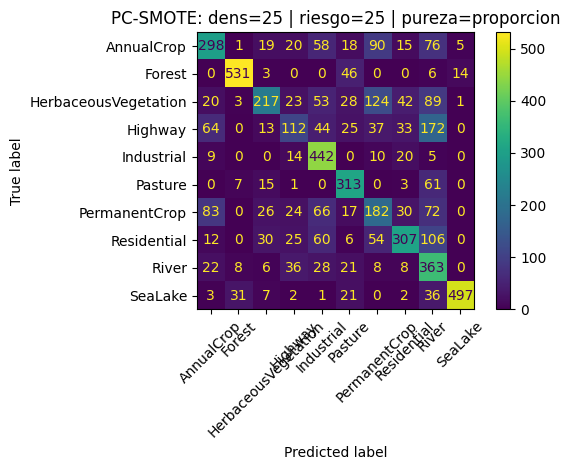
\includegraphics[scale=0.4]{pcsmote_heatmap_best.png}
  \caption{Matriz de confusión para la mejor configuración de PC-SMOTE (densidad=25, riesgo=25, pureza=proporción)}
  \label{fig:pcsmote_best_heatmap}
\end{figure}
